%% smpost/thumbnail/chapter_08_crowd_on_the_road.tex : thumbnail of video 8/30,
%% "Chapter-8 | The Crowd on the Road: Pileup". Motif: one bunch crossing of
%% 2025 seen from the side: the luminous region on the beam line with the
%% vertices of the crowd strung along it, ours the gold star; the b jet leaves
%% our vertex as a cone, its family in red, and strangers from the neighbouring
%% vertices (light grey) walk into it; the crowd's other tracks are faint.
%% Compile: make thumbnails-youtube   (or: pdflatex chapter_08_crowd_on_the_road)
\documentclass[tikz,border=0pt]{standalone}
%% ==========================================================================
%% smpost/thumbnail/thumbnail_common.tex : what every JitJet video thumbnail
%% shares. Each chapter_XX_*.tex in this directory is a standalone TikZ
%% document that \input{}s this file after \documentclass and then draws its
%% own motif on the right of the page.
%%
%% The page is 19.2 cm x 10.8 cm, i.e. 1280 x 720 px at 1 px = 0.015 cm, the
%% YouTube thumbnail size (16:9). `make thumbnails-youtube` compiles every
%% chapter_*.tex here and rasterises it with gs to a 1280 x 720 PNG.
%%
%% Layout: the wordmark top left, the "n / 30" pill top right, the stop number
%% in a milestone ring with the chapter label, the title in two big lines and
%% the subtitle under it, all in the left 10 cm; the motif of the chapter sits
%% in the right part, centred on (\mx, \my), inside about 8 cm x 8 cm, over a
%% soft gold glow.
%%   \thumbbackground
%%   \thumbtext{<stop number>}{<chapter label>}{<n / 30>}{<title, with \\>}{<subtitle>}
%% ==========================================================================
\usepackage[T1]{fontenc}
\usepackage{lmodern}
\usepackage{tgheros}          % TeX Gyre Heros, as on the cover
\usepackage{amssymb}
\usetikzlibrary{calc,arrows.meta,decorations.pathmorphing,decorations.markings,shapes.geometric}
\hyphenpenalty=10000 \exhyphenpenalty=10000   % no hyphens in titles and subtitles

%% -------- palette (identical to cover.tex) ----------------------------------
\definecolor{navy}{HTML}{0B1D3A}
\definecolor{navytop}{HTML}{17365F}
\definecolor{gold}{HTML}{F4B942}
\definecolor{bred}{HTML}{FF5A5A}     % b quark
\definecolor{bblue}{HTML}{6E8EFF}    % bbar
\definecolor{fsr}{HTML}{3DD16E}      % FSR gluons
\definecolor{isr}{HTML}{FF9A3C}      % ISR gluon
\definecolor{hadroncol}{HTML}{FFC24D}
\definecolor{ecalcol}{HTML}{3FBF77}
\definecolor{hcalcol}{HTML}{E58F2A}
\definecolor{steel}{HTML}{9AA7B8}
\definecolor{trackcol}{HTML}{E4ECF7}
\definecolor{pu}{HTML}{8D9AAB}
\definecolor{nucol}{HTML}{5EE7EA}
\definecolor{muoncol}{HTML}{8FB8FF}

%% -------- the cone of the cover, for thumbnails that show it ----------------
\def\kk{0.30}
\pgfmathdeclarefunction{rf}{1}{\pgfmathparse{0.18*#1+0.6*(1+((#1-16.8)/1.2)/sqrt(1+((#1-16.8)/1.2)^2))}}
\pgfmathdeclarefunction{sc}{1}{\pgfmathparse{min(rf(#1)/2.2,1)}}
\newcommand{\xy}[3]{({#1+\kk*#2*sc(#1)*cos(#3)},{#2*sc(#1)*sin(#3)})}
\newcommand{\xring}[2]{%
  \draw[ringback] ({#1},{#2}) arc[start angle=90, end angle=-90, x radius={\kk*#2}, y radius={#2}];
  \draw[ring]     ({#1},{#2}) arc[start angle=90, end angle=270, x radius={\kk*#2}, y radius={#2}];}
\newcommand{\xellipse}[3][]{\path[#1] ({#2},0) ellipse [x radius={\kk*#3}, y radius={#3}];}

%% -------- where the motif goes ----------------------------------------------
\def\mx{14.6}
\def\my{5.3}

%% -------- styles ------------------------------------------------------------
\tikzset{
  ring/.style={draw=gold!75!white, line width=0.6pt, opacity=0.9},
  ringback/.style={draw=white, line width=0.4pt, opacity=0.3, dash pattern=on 1pt off 1pt},
  meridian/.style={draw=white, line width=0.3pt, opacity=0.15},
  edge/.style={draw=gold!80!white, line width=1.1pt},
  bline/.style={draw=bred, line width=3pt, line cap=round},
  bbarline/.style={draw=bblue, line width=3pt, line cap=round},
  qline/.style={draw=trackcol, line width=2pt, line cap=round},
  gluon/.style={draw=fsr, line width=1.6pt, decorate,
    decoration={coil, aspect=0.6, segment length=4pt, amplitude=2.6pt}},
  isrgluon/.style={gluon, draw=isr},
  quark/.style={draw=hadroncol, line width=1.6pt, line cap=round},
  string/.style={draw=hadroncol, line width=2.4pt, line cap=round},
  hadron/.style={circle, fill=hadroncol, draw=navy, line width=0.6pt, inner sep=0pt, minimum size=9pt},
  track/.style={draw=trackcol, line width=1.3pt, line cap=round},
  pudot/.style={circle, fill=pu, inner sep=0pt, minimum size=4pt, opacity=0.8},
  pf/.style={circle, inner sep=0pt, minimum size=5pt, draw=navy, line width=0.3pt},
  roadline/.style={draw=gold, line width=1.4pt, dash pattern=on 7pt off 5pt},
  milestone/.style={circle, draw=gold, fill=navy, line width=1.6pt, minimum size=26pt,
    inner sep=0pt, font=\sffamily\bfseries\large, text=gold},
  mlabel/.style={font=\sffamily\bfseries, text=white, align=center, inner sep=4pt,
    fill=navy, rounded corners=2pt, draw=gold, line width=0.8pt},
  flight/.style={draw=bred, line width=1.4pt, dash pattern=on 4pt off 3pt},
  vertex/.style={circle, draw=bred, fill=navy, line width=1.6pt, inner sep=0pt, minimum size=9pt},
  arrowg/.style={-{Stealth[length=7pt]}, draw=gold, line width=1.2pt},
  motiflabel/.style={font=\sffamily\bfseries\small, inner sep=1.5pt},
}

%% -------- the page ----------------------------------------------------------
\newcommand{\thumbbackground}{%
  \useasboundingbox (0,0) rectangle (19.2,10.8);
  \clip (0,0) rectangle (19.2,10.8);
  \shade[top color=navytop, bottom color=navy!80!black] (0,0) rectangle (19.2,10.8);
  \draw[white, opacity=0.045, line width=0.3pt, step=1cm] (0,0) grid (19.2,10.8);
  \shade[inner color=gold, outer color=navy, opacity=0.16] (\mx,\my) circle[radius=4.6];
  \draw[gold, line width=0.6pt, opacity=0.8] (0.9,0.85) -- (18.3,0.85);
  \node[anchor=south west, gold!80!white, font=\sffamily\scriptsize] at (0.9,0.95) {Journey Is The Jet \,$\cdot$\, bottom to top};
  \node[anchor=south east, white!70!navy, font=\sffamily\scriptsize] at (18.3,0.95) {github.com/ravindkv/JitJet};
}

%% \thumbtext{stop}{chapter label}{n / 30}{title}{subtitle}
\newcommand{\thumbtext}[5]{%
  \node[anchor=west] at (0.9,9.65)
    {\fontsize{26}{28}\selectfont\sffamily\bfseries{\color{white}Jit}{\color{gold}Jet}};
  \node[anchor=east, gold, font=\sffamily\bfseries\small, draw=gold, line width=0.8pt,
        rounded corners=6pt, inner xsep=7pt, inner ysep=3.5pt] at (18.3,9.65) {#3};
  \node[milestone] (stop) at (1.45,7.85) {#1};
  \node[anchor=west, gold, font=\fontsize{15}{17}\selectfont\sffamily\scshape] at (2.1,7.85) {#2};
  \node[anchor=north west, white, align=left, inner sep=0pt,
        font=\fontsize{34}{39}\selectfont\sffamily\bfseries] (ttl) at (0.9,7.05) {#4};
  \node[anchor=north west, gold!90!white, align=left, inner sep=0pt, text width=9.6cm,
        font=\fontsize{14}{17}\selectfont\sffamily\itshape] at ($(ttl.south west)+(0,-0.4)$) {#5};
}

\begin{document}
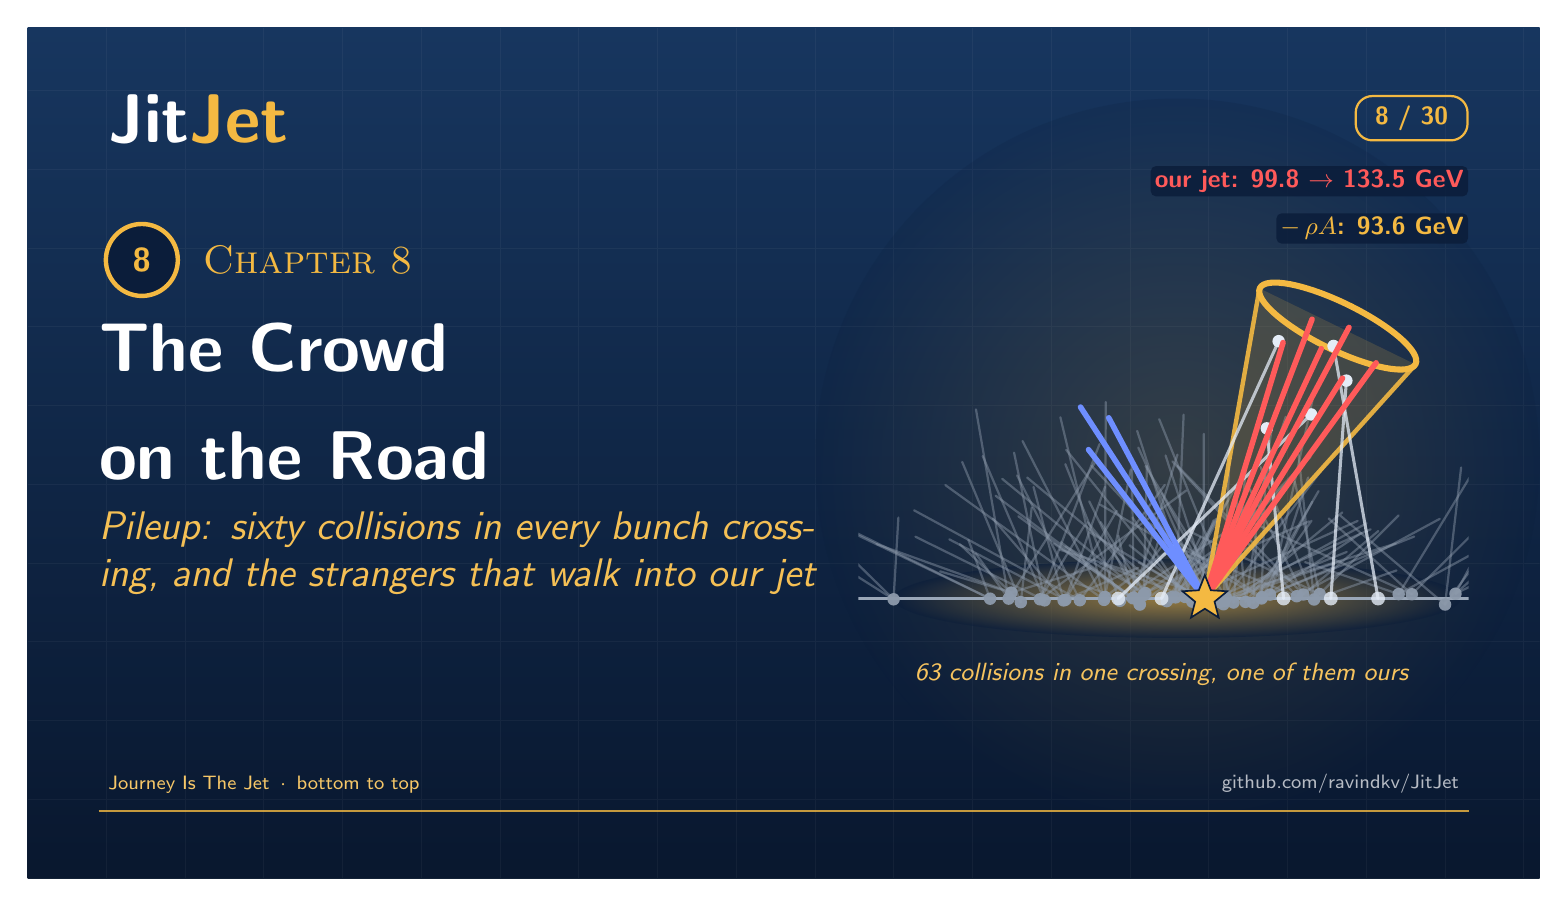
\begin{tikzpicture}[x=1cm,y=1cm]
\thumbbackground
\thumbtext{8}{Chapter 8}{8 / 30}{The Crowd\\on the Road}{Pileup: sixty collisions in every bunch crossing, and the strangers that walk into our jet}

\begin{scope}[shift={(\mx,\my)}]
\def\by{-1.75}    % the beam line
\def\vx{0.35}     % our vertex
%% everything the crowd draws stays in the motif box
\begin{scope}
\clip (-4.05,-3.3) rectangle (3.7,3.75);
%% the luminous region on the beam line
\shade[inner color=gold, outer color=navy, opacity=0.55] (0,\by) ellipse [x radius=3.6, y radius=0.5];
\draw[steel, line width=1.4pt] (-4.6,\by) -- (4.3,\by);
%% the crowd: vertices along the beam, each with a few faint tracks
\pgfmathsetseed{60}
\foreach \i in {1,...,46}{
  \pgfmathsetmacro{\zz}{1.35*(rnd+rnd+rnd-1.5)*2}
  \pgfmathsetmacro{\yy}{\by+0.16*(rnd-0.5)}
  \foreach \k in {1,2,3}{
    \pgfmathsetmacro{\aa}{15+150*rnd}
    \pgfmathsetmacro{\ll}{0.7+1.9*rnd}
    \draw[pu, opacity=0.45, line width=0.8pt, line cap=round] (\zz,\yy) -- ++(\aa:\ll);}
  \node[pudot, minimum size=4.5pt, opacity=0.95] at (\zz,\yy) {};}
\end{scope}
%% our b jet: a cone from our vertex, its cap a circle seen at an angle
\coordinate (V) at (\vx,\by);
\coordinate (C) at ($(V)+(64:3.85)$);
\fill[gold, opacity=0.16] (V) -- ($(V)+(48:4.0)$) -- ($(V)+(80:4.0)$) -- cycle;
\draw[gold, line width=1.6pt, opacity=0.9] (V) -- ($(V)+(48:4.0)$) (V) -- ($(V)+(80:4.0)$);
\draw[gold, line width=2.2pt, rotate around={-26:(C)}] (C) ellipse [x radius=1.1, y radius=0.3];
%% strangers from the neighbouring vertices walking into the cone
\foreach \sx/\a/\d in {-0.75/60/2.7, 1.35/70/2.3, 1.95/57/3.3, -0.2/74/3.4, 2.55/63/3.6}{
  \draw[trackcol, line width=1.1pt, line cap=round, opacity=0.75] (\sx,\by) -- ($(V)+(\a:\d)$);
  \node[circle, fill=trackcol, inner sep=0pt, minimum size=4.5pt] at ($(V)+(\a:\d)$) {};
  \node[pudot, fill=trackcol, minimum size=5pt] at (\sx,\by) {};}
%% the family: the mother's tracks inside the cone, and the bbar jet the other way
\foreach \a/\l in {54/3.7, 58/3.3, 62/3.9, 65/3.5, 69/3.8, 73/3.4}
  \draw[bred, line width=2pt, line cap=round] (V) -- ++(\a:\l);
\foreach \a/\l in {118/2.6, 123/2.9, 128/2.4}
  \draw[bblue, line width=2pt, line cap=round] (V) -- ++(\a:\l);
%% our collision
\node[star, star points=5, star point ratio=2.3, fill=gold, draw=navy, line width=0.6pt, inner sep=0pt, minimum size=17pt] at (V) {};
\end{scope}
%% the numbers to take away
\node[bred, motiflabel, anchor=north east, fill=navy, fill opacity=0.85, text opacity=1, rounded corners=2pt, align=right] at (18.3,9.05)
  {our jet: 99.8 $\to$ 133.5 GeV};
\node[gold, motiflabel, anchor=north east, fill=navy, fill opacity=0.85, text opacity=1, rounded corners=2pt, align=right] at (18.3,8.45)
  {$-\,\rho A$: 93.6 GeV};
\node[gold!85!white, font=\sffamily\small\itshape, anchor=north] at (\mx-0.2,\my-2.45)
  {63 collisions in one crossing, one of them ours};
\end{tikzpicture}
\end{document}
